\subsection{Data Reduction Studies}
\label{subsec:pmc-results-data-reduction-studies}

\EB{Acho que seria bom usar um título mais específico. Algo como: "Training Set Size", "Training Set Reduction Studies", "Impact of training set size"...}

This section discusses how predictive accuracy changes when the training dataset is subsampled, thus reducing the total number of configurations.
The aim is to identify whether smaller subsets of shape–memory measurements can still produce reliable models.
Specifically, experiments removed “middle-range” samples of the volume dimension (or shape parameters more broadly), keeping the smallest and largest volumes, while uniformly discarding intermediate sizes.
Both Envelope and \ac{GST3D} used the best models identified (Gradient Boosting and Decision Tree, respectively), while Gaussian Filter used Linear Regression.

\EB{Esta seção é bem interessante e importante. No entanto, a decisão de usar volumes pequenos e grandes em vez de pequenos e médios me pareceu arbitrária. Em tese, seria melhor usar pequenos e médios, já que o custo de coletar estes dados é menor.}

\subsubsection{Subsampling Strategy and Motivation}
\label{subsec:data-reduction-strategy-and-motivation}

The data-reduction procedure systematically excludes shape configurations from the central volume interval, retaining the extremes that often yield the highest or lowest memory usage.
By gradually lowering the sample count (\(N\)), it is possible to observe how model performance deteriorates or remains stable.
Figures~\ref{fig:cross_data_reduction_and_residual}--\ref{fig:metrics_evolution_sample_size_operators} present the overall results.
Figure~\ref{fig:cross_data_reduction_and_residual}(a) plots the \ac{RMSE} as a function of sample size, while part~(b) shows how residual-based metrics evolve.
All three operators suffer performance degradation under severe reductions, but moderate cutbacks can still yield acceptable accuracy.

\begin{figure*}[htbp]
    \centering
    \begin{subfigure}[t]{0.49\textwidth}
        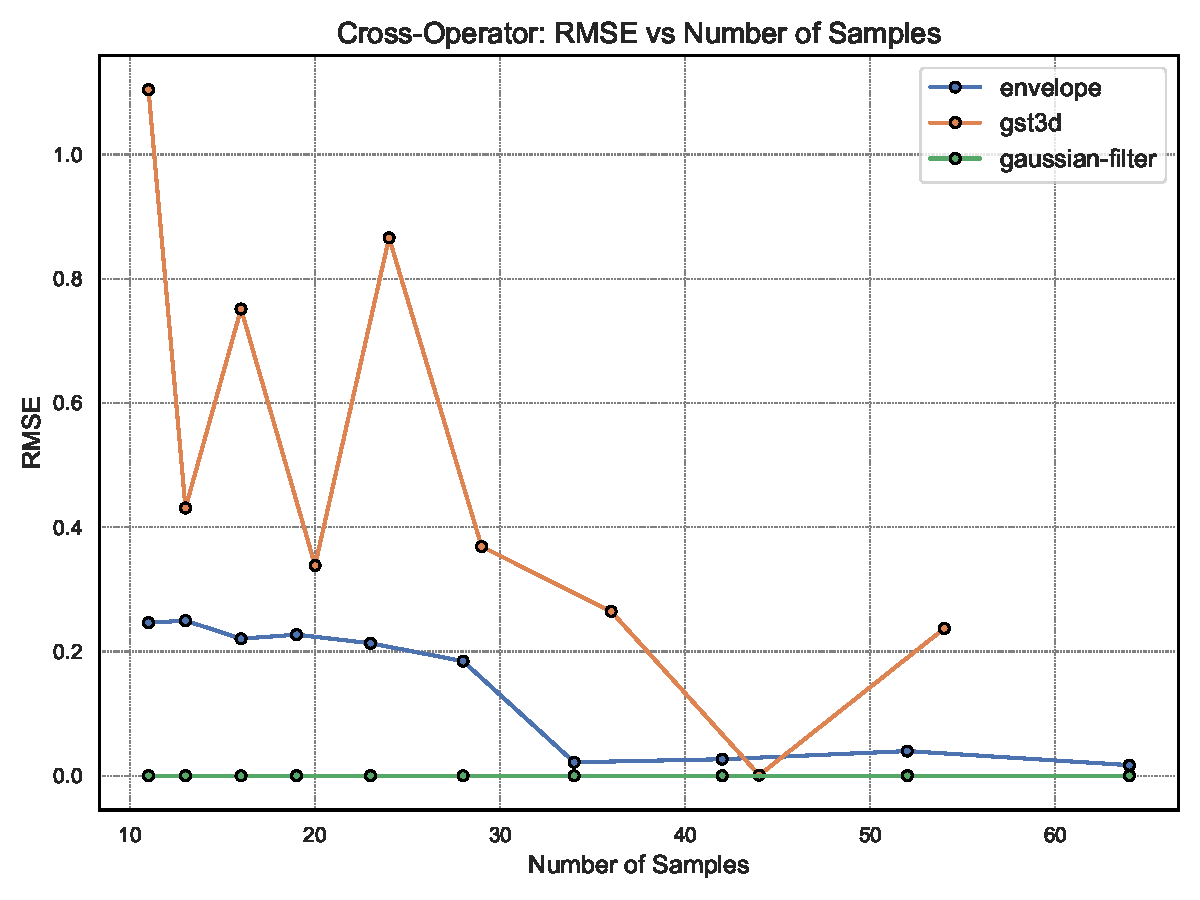
\includegraphics[width=\textwidth]{assets/images/05/cross_data_reduction_rmse}
        \caption{\ac{RMSE} across Envelope, \ac{GST3D}, and Gaussian Filter as sample size decreases.
        A smooth upward trend reflects the increasing difficulty of fitting with fewer examples.
        \EB{Por que escolheu o RMSE em vez do outro score?}
        }
    \end{subfigure}
    \hfill
    \begin{subfigure}[t]{0.49\textwidth}
        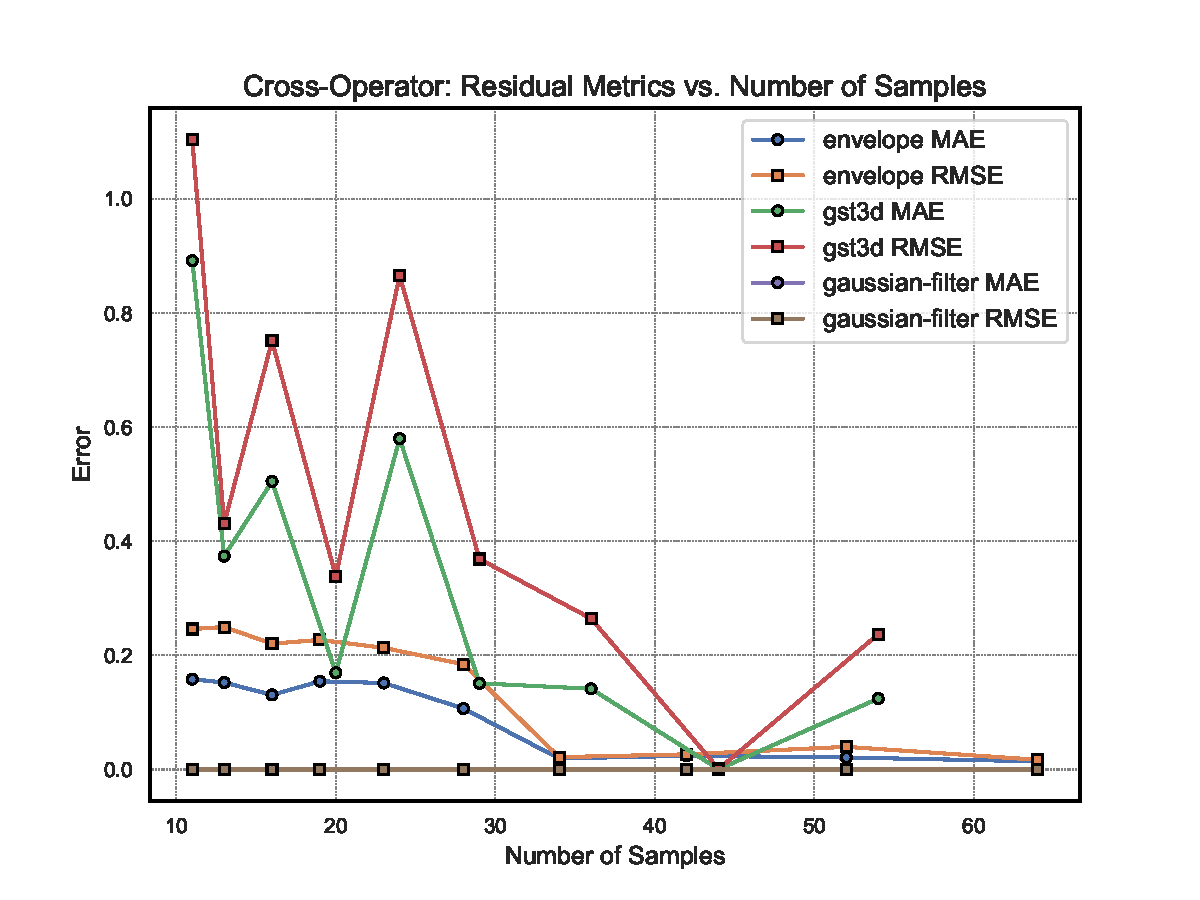
\includegraphics[width=\textwidth]{assets/images/05/residual_metrics_by_sample_size}
        \caption{Residual metrics also climb with smaller datasets.
        Minimal sets (\(<20\) samples) show large spikes, indicating insufficient coverage of intermediate volumes.}
    \end{subfigure}
    \caption{Data-reduction effects, viewed globally for all operators.
    Reducing the training set drives up errors and variability.
    \EB{Estes dois gráficos são bem parecidos. Faz sentido manter os dois. Talvez o da esquerda já seja suficiente.}
    \label{fig:cross_data_reduction_and_residual}
    }
\end{figure*}

\subsubsection{Operator-Wise Performance Trends}
\label{subsec:operator-wise-sample-size-analysis}

Figures~\ref{fig:residual_metrics_by_sample_size_operators}--\ref{fig:metrics_evolution_sample_size_operators} elaborate on each operator individually.
When sample sizes fall below roughly 30, \ac{RMSE}, \ac{MAE}, and residual variance begin to rise more sharply.
This pattern is consistent with the notion that “filling in” the middle range of volumes is essential for maintaining a robust regression fit.
However, moderately pruned datasets (e.g., 40–50 samples) still achieve respectable $R^2 > 0.98$ in most cases, as verified by the CSV results in Table~\ref{tab:data_reduction_summary}.

\begin{figure*}[htbp]
    \centering
    \begin{subfigure}[t]{0.32\textwidth}
        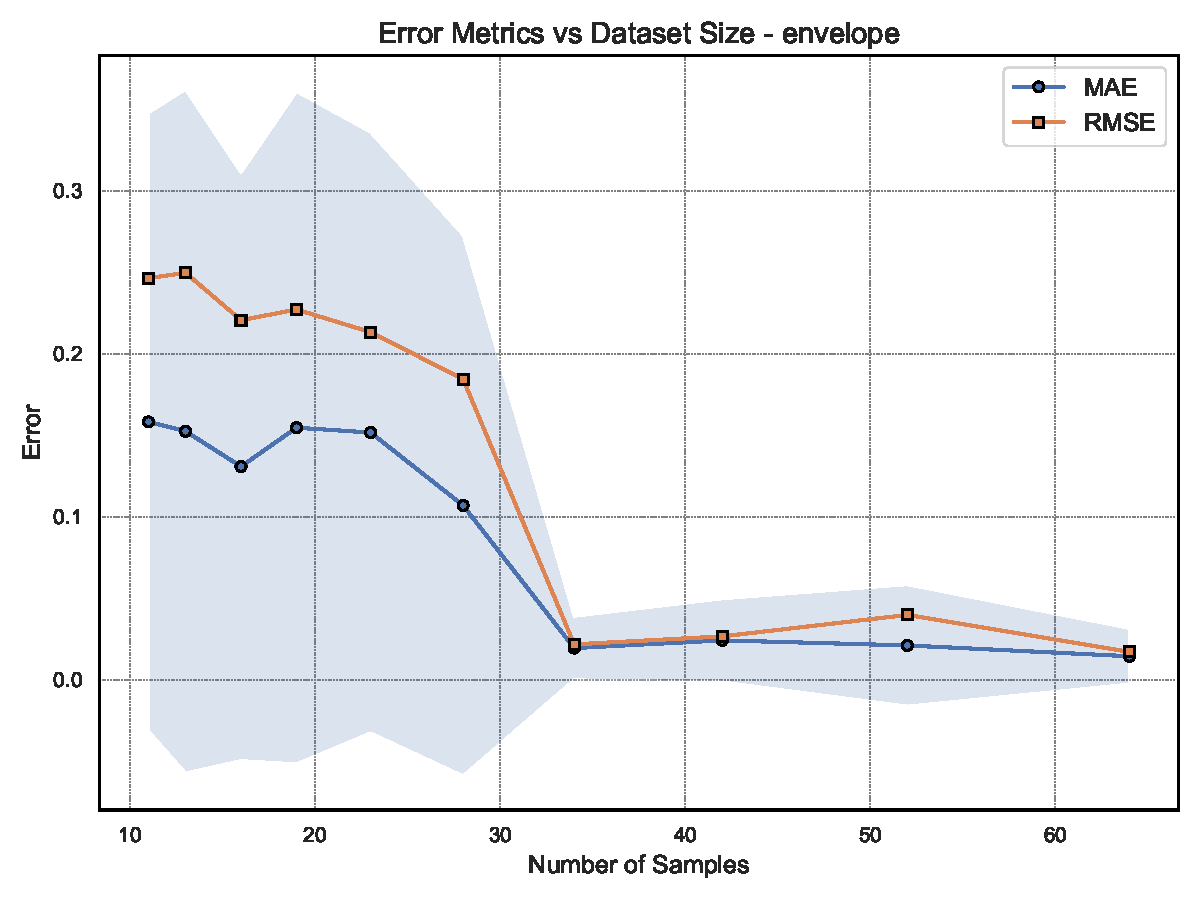
\includegraphics[width=\textwidth]{assets/images/05/residual_metrics_by_sample_size_envelope}
        \caption{Envelope}
    \end{subfigure}
    \hfill
    \begin{subfigure}[t]{0.32\textwidth}
        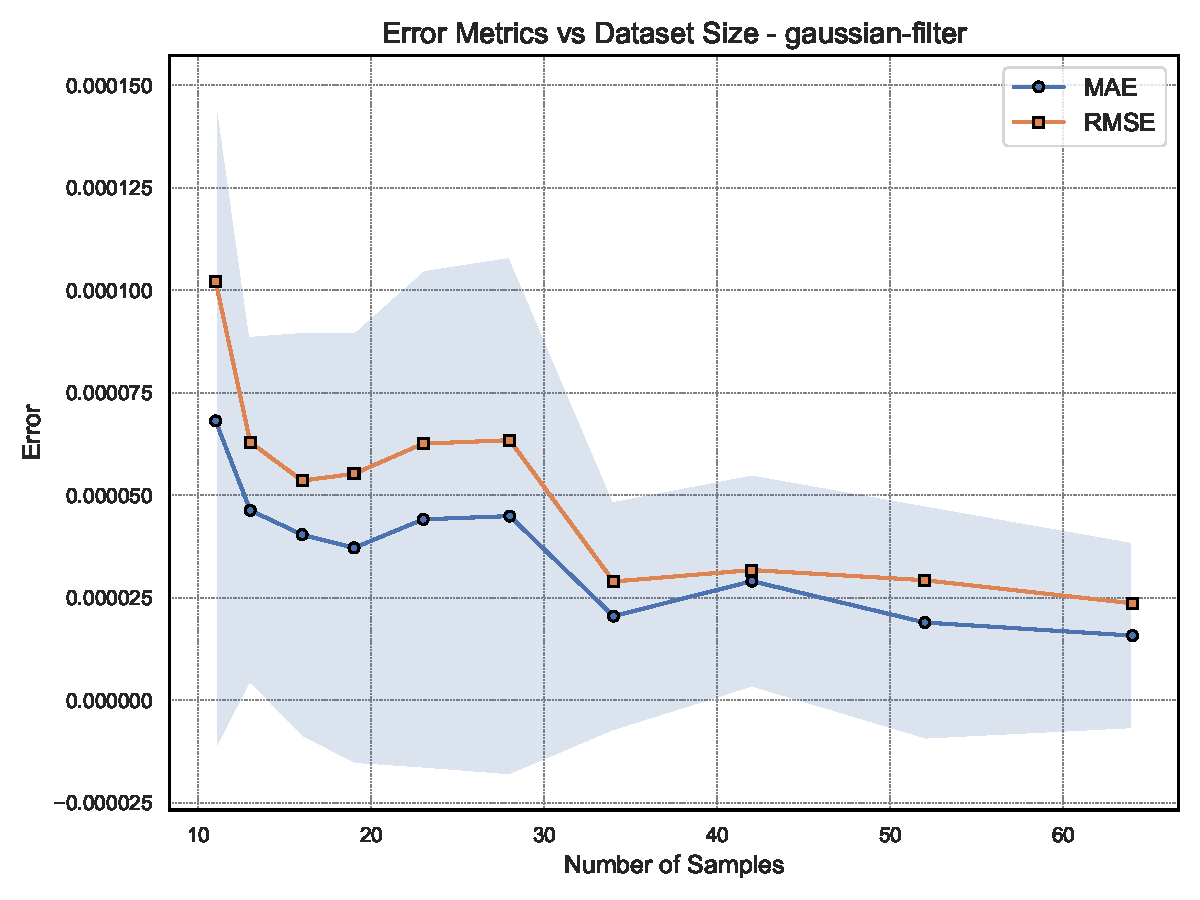
\includegraphics[width=\textwidth]{assets/images/05/residual_metrics_by_sample_size_gaussian-filter}
        \caption{Gaussian Filter}
    \end{subfigure}
    \hfill
    \begin{subfigure}[t]{0.32\textwidth}
        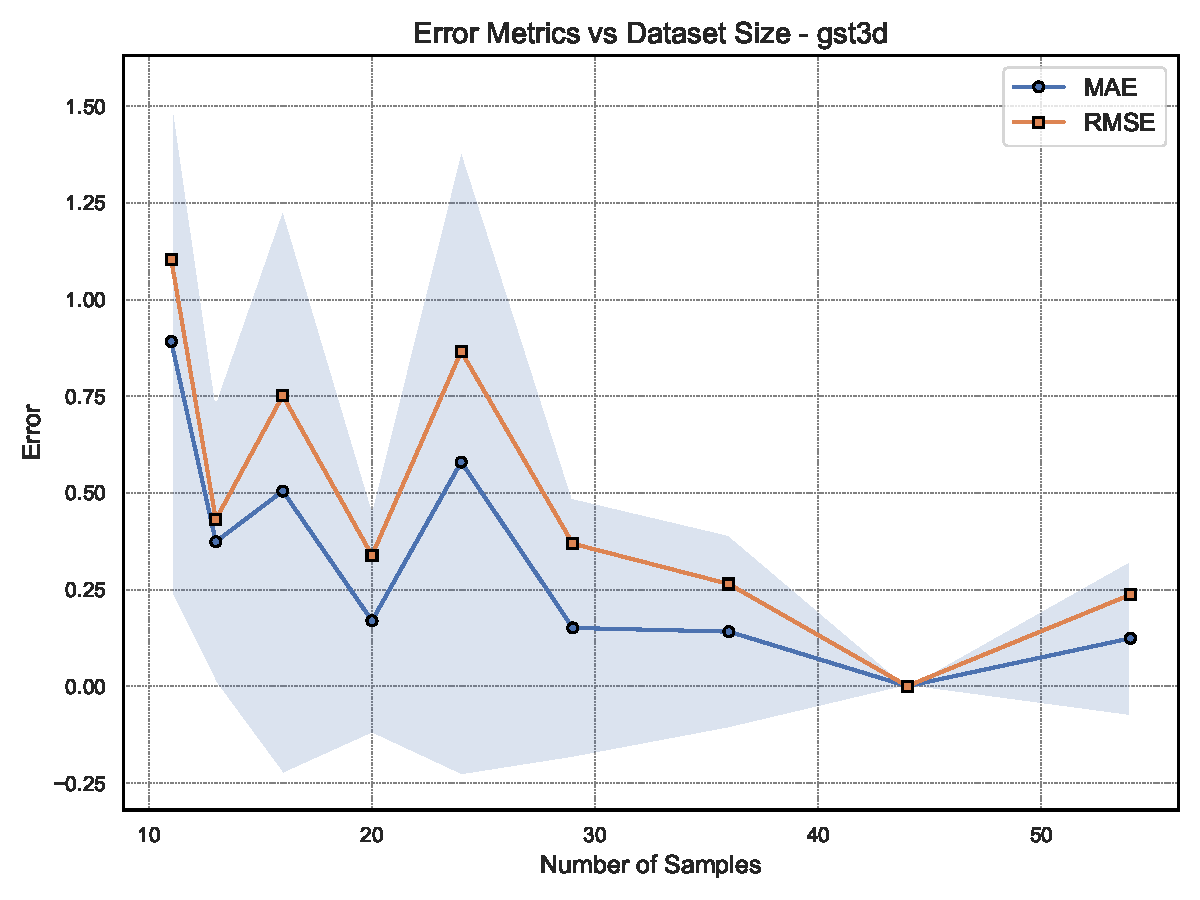
\includegraphics[width=\textwidth]{assets/images/05/residual_metrics_by_sample_size_gst3d}
        \caption{\ac{GST3D}}
    \end{subfigure}
    \caption{Residual-based metrics per operator as sample size diminishes.
    Error bars reflect increasing variability at smaller dataset sizes.}
    \label{fig:residual_metrics_by_sample_size_operators}
\end{figure*}

\begin{figure*}[htbp]
    \centering
    \begin{subfigure}[t]{0.32\textwidth}
        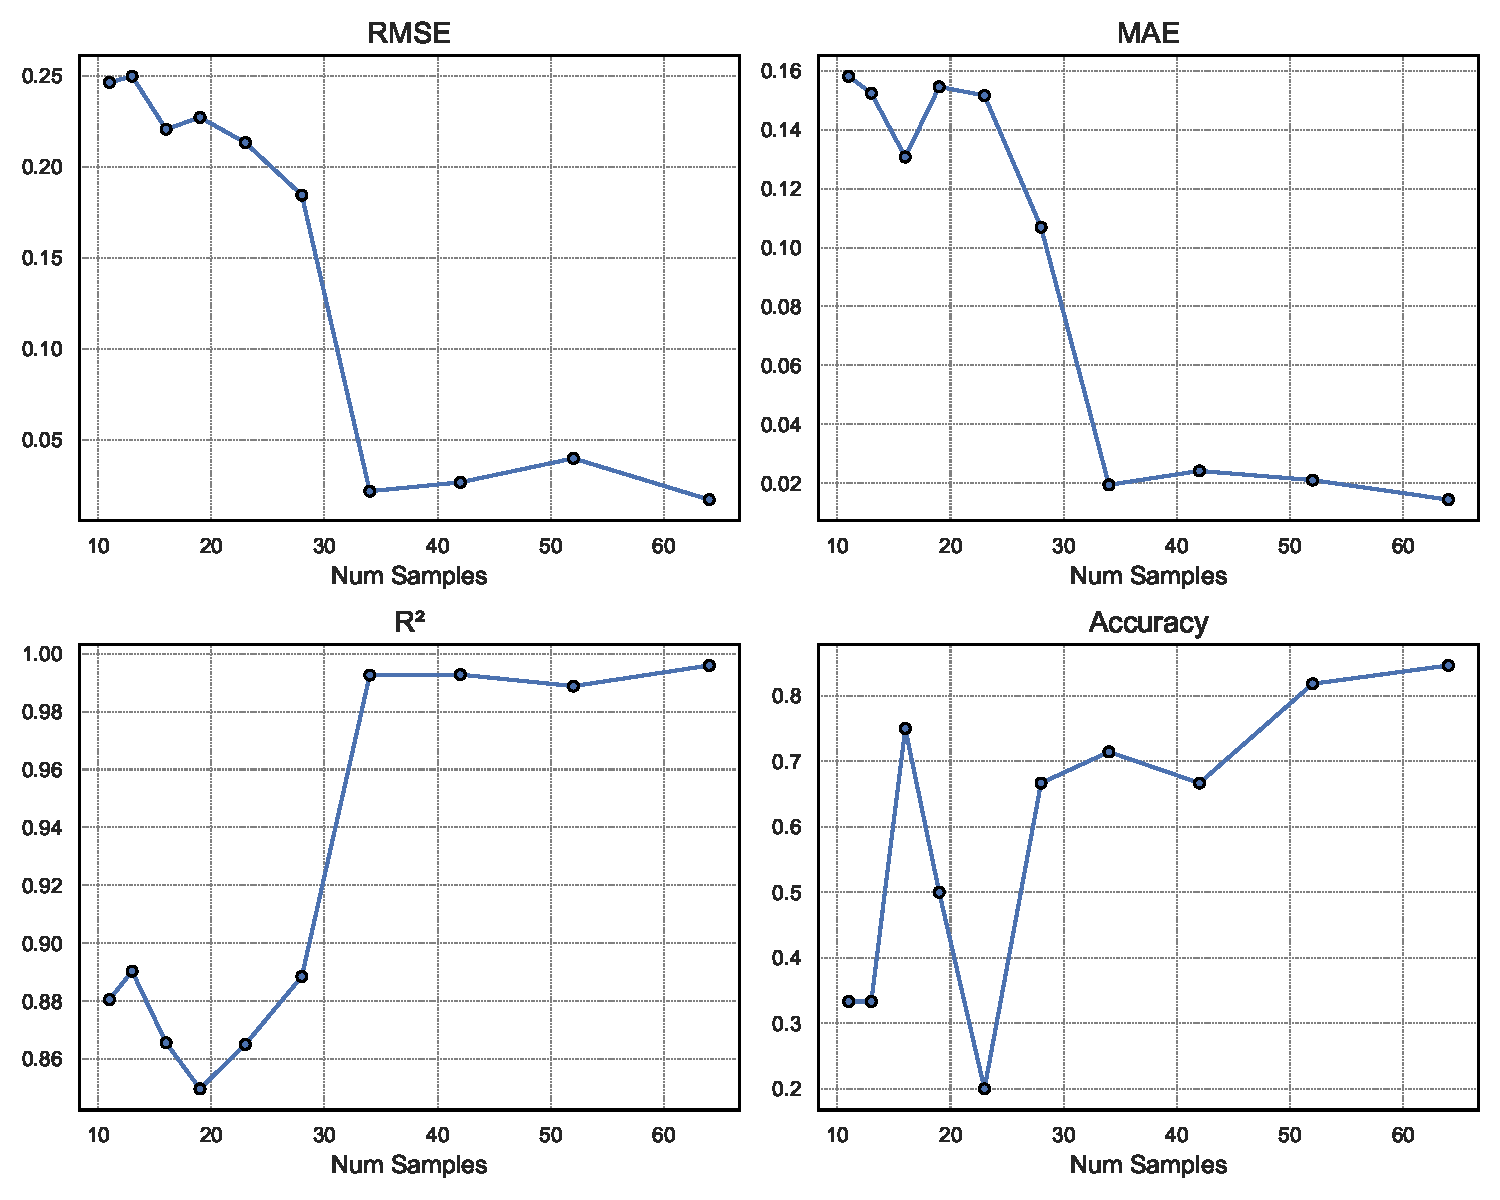
\includegraphics[width=\textwidth]{assets/images/05/metrics_evolution_by_sample_size_envelope}
        \caption{Envelope}
    \end{subfigure}
    \hfill
    \begin{subfigure}[t]{0.32\textwidth}
        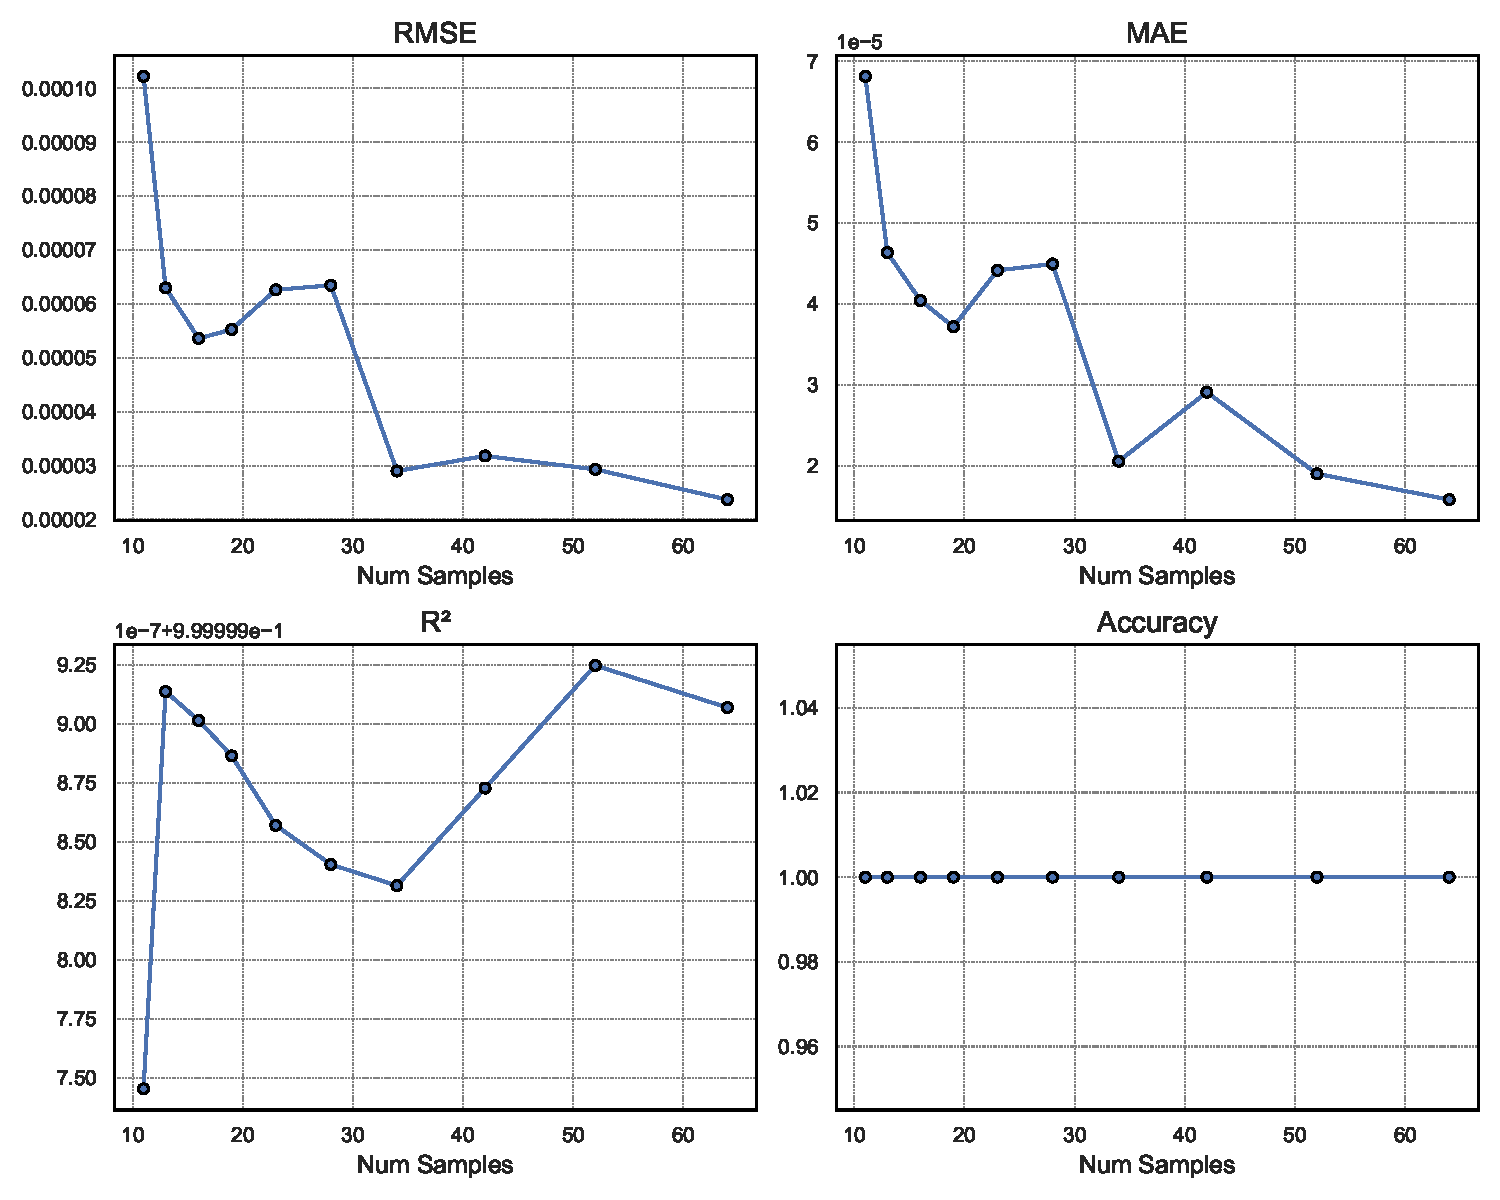
\includegraphics[width=\textwidth]{assets/images/05/metrics_evolution_by_sample_size_gaussian-filter}
        \caption{Gaussian Filter}
    \end{subfigure}
    \hfill
    \begin{subfigure}[t]{0.32\textwidth}
        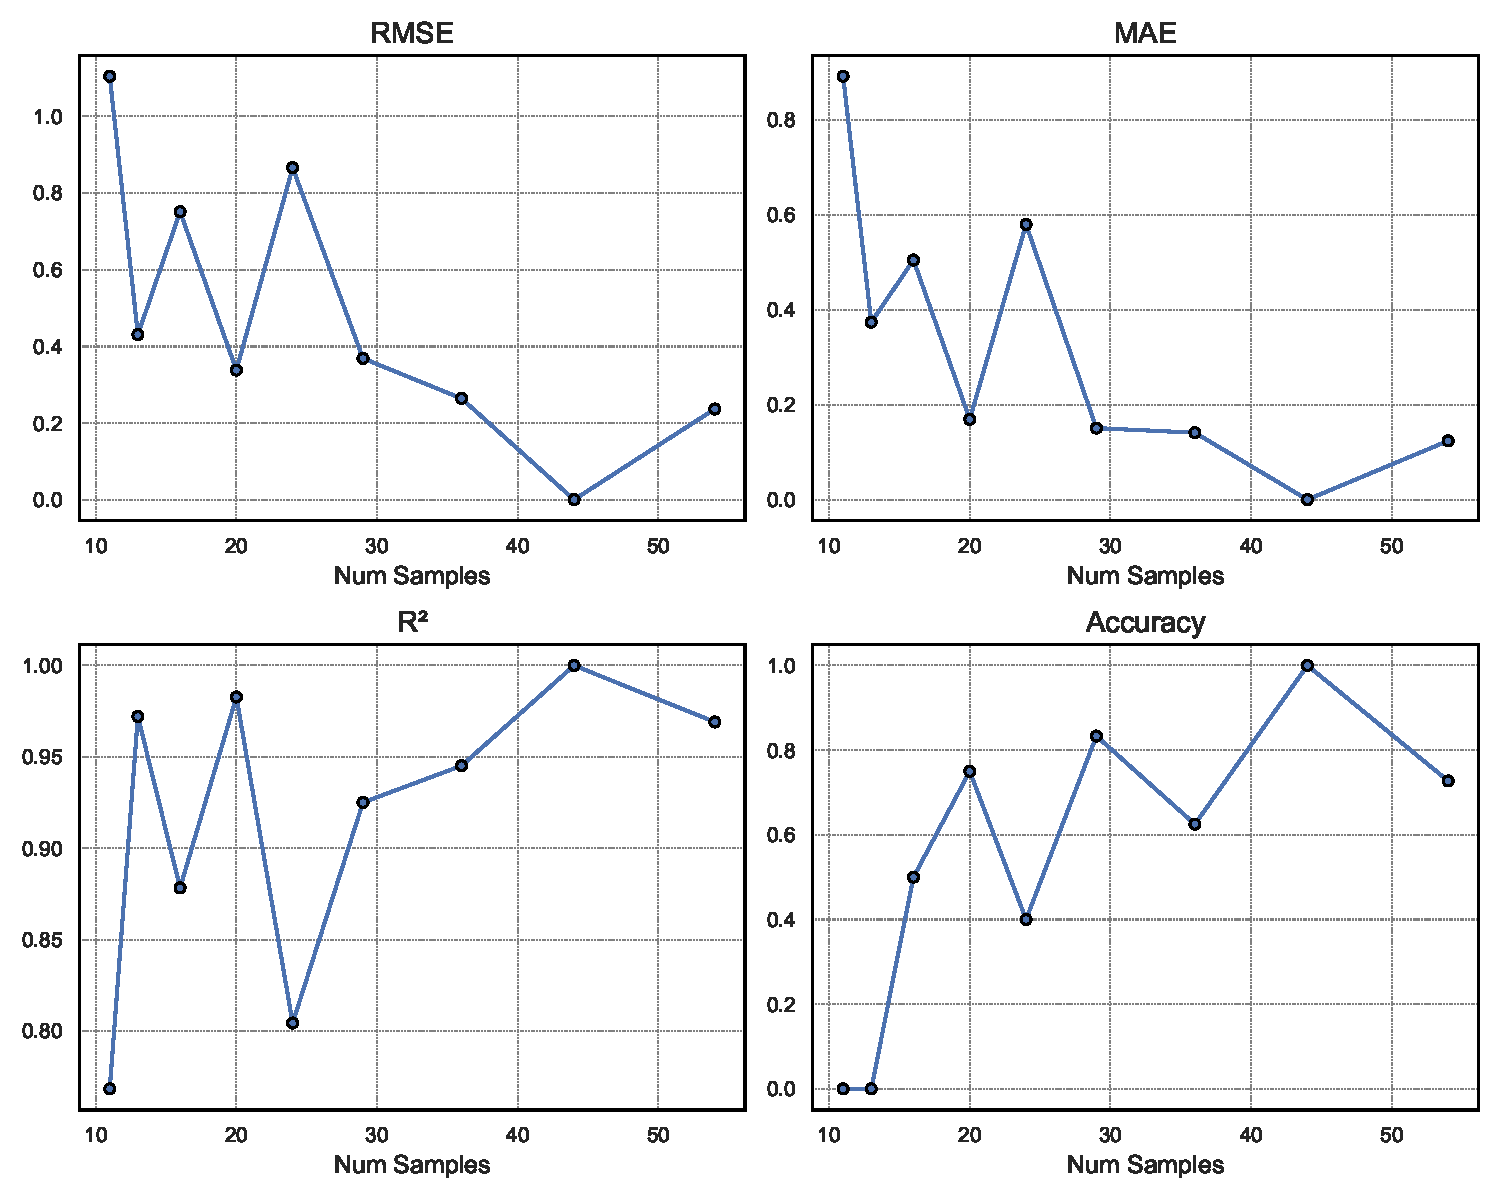
\includegraphics[width=\textwidth]{assets/images/05/metrics_evolution_by_sample_size_gst3d}
        \caption{\ac{GST3D}}
    \end{subfigure}
    \caption{All metrics tracked as sample sizes drop, plotted per operator.
    \ac{RMSE} and \ac{MAE} grow steadily, while $R^2$ and accuracy decline.}
    \label{fig:metrics_evolution_sample_size_operators}
\end{figure*}

\subsubsection{Score Comparisons and Sweet Spot Around 30 Samples}
\label{subsec:score-comparisons-and-sweet-spot}

Figures~\ref{fig:score_by_sample_size_operators}(a)–(c) plot the consolidated “score” metric described in Section~\ref{subsec:pmc-results-model-performance-overview}.
All three operators see an inflection around 30–35 samples where model quality remains strong.
Below that threshold, the curves dip more significantly, reflecting the loss of mid-range volume coverage.
Above 40–50 samples, the gains saturate, and further additions of similar configurations do not yield major improvements.

\begin{figure*}[htbp]
    \centering
    \begin{subfigure}[t]{0.32\textwidth}
        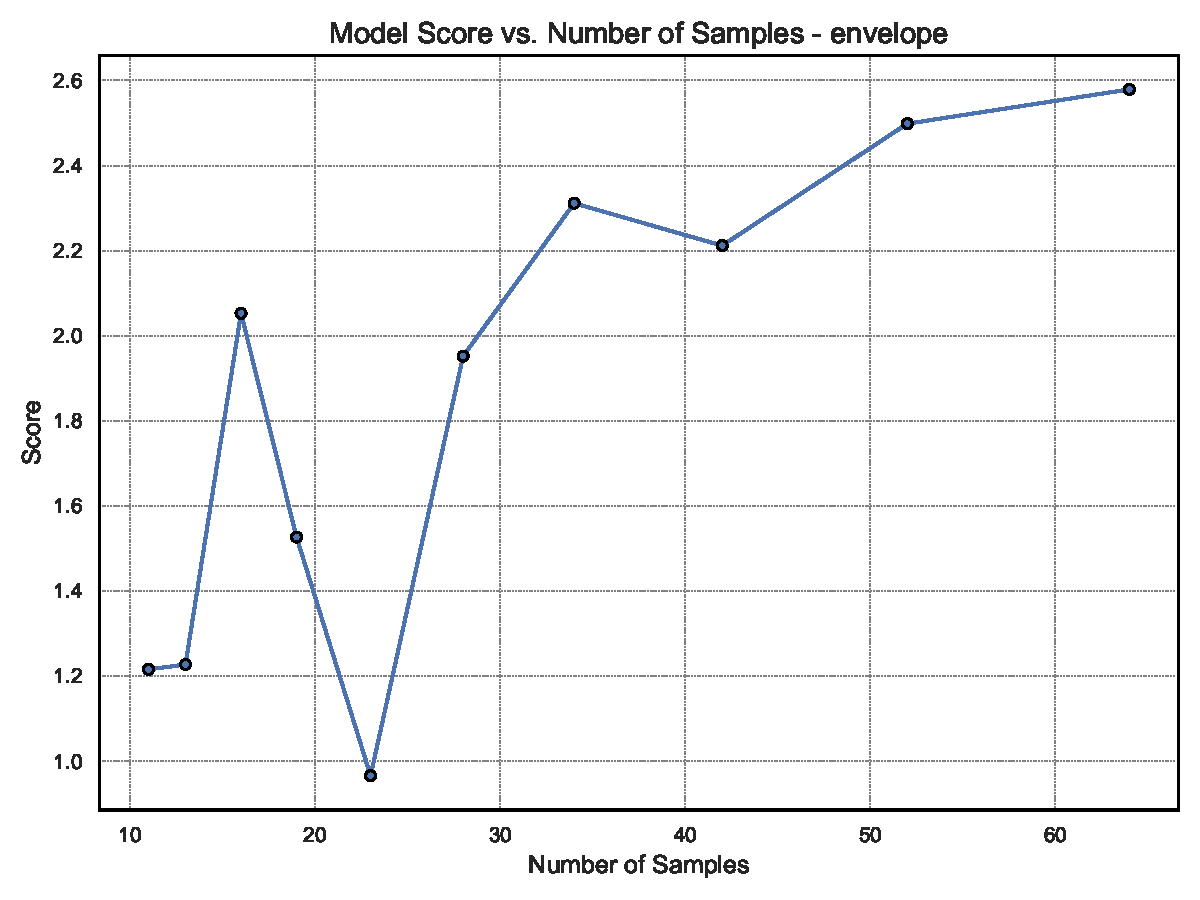
\includegraphics[width=\textwidth]{assets/images/05/score_by_sample_size_envelope}
        \caption{Envelope}
    \end{subfigure}
    \hfill
    \begin{subfigure}[t]{0.32\textwidth}
        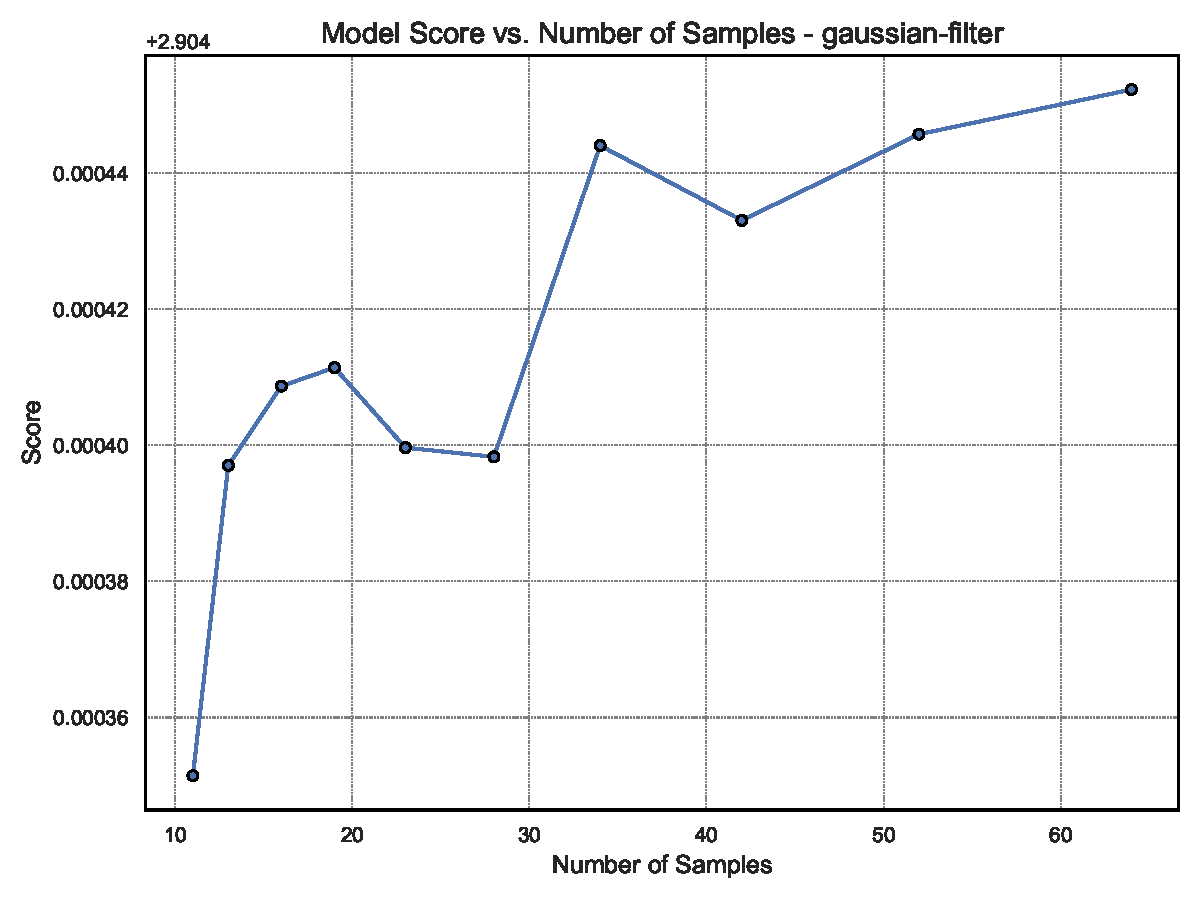
\includegraphics[width=\textwidth]{assets/images/05/score_by_sample_size_gaussian-filter}
        \caption{Gaussian Filter}
    \end{subfigure}
    \hfill
    \begin{subfigure}[t]{0.32\textwidth}
        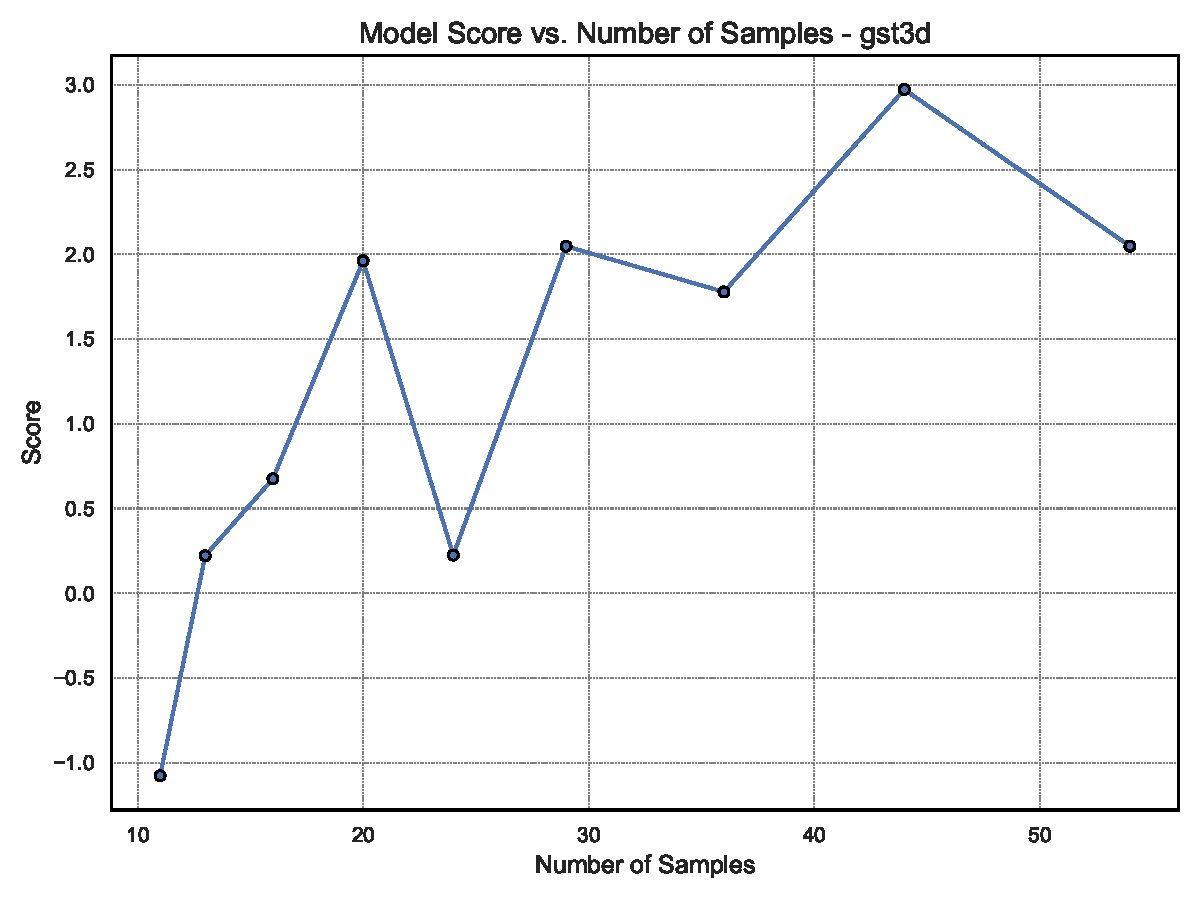
\includegraphics[width=\textwidth]{assets/images/05/score_by_sample_size_gst3d}
        \caption{\ac{GST3D}}
    \end{subfigure}
    \caption{Model scores vs.\ sample size.
    Each operator shows a notable decline below \(\sim\)30 samples, marking a practical lower bound for training.}
    \label{fig:score_by_sample_size_operators}
\end{figure*}

Table~\ref{tab:data_reduction_summary} illustrates partial data from the CSV files.
It includes selected sample sizes and the resulting \ac{RMSE}, $R^2$, accuracy, and overall score.
Even moderate subsampling (34 or 42 samples, for instance) still achieves high $R^2$ for Envelope and Gaussian Filter.
\ac{GST3D} remains more sensitive, though a subset of 44 samples can deliver near-perfect accuracy.

\begin{table}[htbp]
    \centering
    \begin{tabular}{lccccc}
        \hline
        \textbf{Operator} & \textbf{\#Samples} & \textbf{\ac{RMSE}}    & \textbf{$R^2$} & \textbf{Accuracy} & \textbf{Score} \\
        \hline
        \multirow{3}{*}{\textbf{Envelope}}
        & 64                 & 0.0170                & 0.9959         & 0.8462            & 2.5789         \\
        & 34                 & 0.0217                & 0.9926         & 0.7143            & 2.3113         \\
        & 11                 & 0.2463                & 0.8805         & 0.3333            & 1.2155         \\
        \hline
        \multirow{3}{*}{\textbf{Gaussian Filter}}
        & 64                 & \(2.37\times10^{-5}\) & 0.9999999      & 1.0               & 2.9045         \\
        & 34                 & \(2.90\times10^{-5}\) & 0.9999998      & 1.0               & 2.9044         \\
        & 11                 & \(1.02\times10^{-4}\) & 0.9999997      & 1.0               & 2.9044         \\
        \hline
        \multirow{3}{*}{\textbf{\ac{GST3D}}}
        & 54                 & 0.2371                & 0.9691         & 0.7273            & 2.0478         \\
        & 29                 & 0.3689                & 0.9251         & 0.8333            & 2.0472         \\
        & 11                 & 1.1042                & 0.7684         & 0.0000            & -1.0768        \\
        \hline
    \end{tabular}
    \caption{Selected data-reduction results (largest, close to 30, smallest) for each operator.
    Subsets of around 30--40 samples retain robust accuracy, while very small sets
        (e.g., 11) cause steep performance declines, especially for \ac{GST3D}.}
    \label{tab:data_reduction_summary}
\end{table}

\subsubsection{Conclusions on Data Pruning}
\label{subsec:data-reduction-conclusions}

These experiments confirm that seismic-memory models require at least 30 samples to maintain stable performance, primarily to capture mid-scale volumes.
Envelope and Gaussian Filter remain accurate even with moderate data pruning, while \ac{GST3D} is somewhat more sensitive due to its heavier internal complexity.
Still, collecting 30–40 shape configurations seems sufficient for building robust predictive models without incurring excessive data-gathering overhead.
Subsequent sections integrate these findings with the feature-selection insights to propose minimal yet effective training strategies for real-world \ac{HPC} applications.